\documentclass[landscape,a0paper,fontscale=0.282]{baposter}

\usepackage[vlined]{algorithm2e}
\usepackage{times}
\usepackage{calc}
\usepackage{url}
\usepackage[spanish]{babel}
\usepackage[utf8]{inputenc}
\usepackage{graphicx}
\usepackage{amsmath}
\usepackage{amssymb}
\usepackage{relsize}
\usepackage{multirow}
\usepackage{booktabs}

\usepackage{graphicx}
\usepackage{multicol}
\usepackage[T1]{fontenc}
\usepackage{ae}

\graphicspath{{images/}}

\definecolor{bordercol}{RGB}{210,210,240}
\definecolor{headercol1}{RGB}{0,0,0}
\definecolor{headercol2}{RGB}{51,255,255}
\definecolor{headerfontcol}{RGB}{250,250,250}
\definecolor{boxcolor}{RGB}{250,255,250}
\definecolor{darkgreen}{RGB}{0,153,0}

%%%%%%%%%%%%%%%%%%%%%%%%%%%%%%%%%%%%%%%%%%%%%%%%%%%%%%%%%%%%%%%%%%%%%%%%%%%%%
%% Begin of Document
%%%%%%%%%%%%%%%%%%%%%%%%%%%%%%%%%%%%%%%%%%%%%%%%%%%%%%%%%%%%%%%%%%%%%%%%%%%%%
\begin{document}
	%%% Setting Background Image %%%%%%%%%%%%%%%%%%%%%%%%%%%%%%%%%%%%%%%%%%%%%%%%%%
	\background{
		\begin{tikzpicture}[remember picture,overlay]%
		\draw (current page.north west)+(-2em,2em) node[anchor=north west]
		{\includegraphics[height=1.1\textheight]{background}};
		\end{tikzpicture}
	}
	
%%%%%%%%%%%%%%%%%%%%%%%%%%%%%%%%%%%%%%%%%%%%%%%%%%%%%%%%%%%%%%%%%%%%%%%%%%%%%
%% Here starts the poster
%%---------------------------------------------------------------------------
%% Format it to your taste with the options
%%%%%%%%%%%%%%%%%%%%%%%%%%%%%%%%%%%%%%%%%%%%%%%%%%%%%%%%%%%%%%%%%%%%%%%%%%%%%
\begin{poster}{
		grid=false,
		% Option is left on true though the eyecatcher is not used. The reason is
		% that we have a bit nicer looking title and author formatting in the headercol
		% this way
		eyecatcher=true, 
		borderColor=bordercol,
		headerColorOne=headercol1,
		headerColorTwo=headercol2,
		headerFontColor=headerfontcol,
		% Only simple background color used, no shading, so boxColorTwo isn't necessary
		boxColorOne=boxcolor,
		headershape=roundedright,
		headerfont=\Large\sf\bf,
		textborder=roundedleft,
		background=user,
		headerborder=open,
		boxshade=plain
	}
 % Eye Catcher
 {
      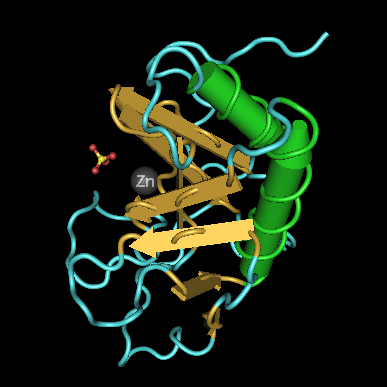
\includegraphics[width=0.09\linewidth]{shh_protein}
 }
 % Title
 {\sf \Huge Nuevo modelo para el sistema de señalización de Shh}
 % Authors
 {Bartolomé Ortiz Viso - \texttt{bortiz@correo.ugr.es} \\ \textit{Tutor: Óscar Sánchez Romero -  \texttt{osscanhe@ugr.es}}}
 % University logo
 {
  \begin{tabular}{r}
    \includegraphics[height=0.12\textheight]{logougr}\\
  \end{tabular}
 }

%%%%%%%%%%%%%%%%%%%%%%%%%%%%%%%%%%%%%%%%%%%%%%%%%%%%%%%%%%%%%%%%%%%%%%%%%%%%%%
  \headerbox{Motivación y Objetivo}{name=motivation,column=0,row=0,span=1}{
%%%%%%%%%%%%%%%%%%%%%%%%%%%%%%%%%%%%%%%%%%%%%%%%%%%%%%%%%%%%%%%%%%%%%%%%%%%%%%
   Shh es una proteína \textbf{esencial} durante la especialización celular en animales como el ratón. La presencia y cantidad de esta molécula en el medio extracelular desemboca en una \textbf{compleja cascada biológica} que influye en procesos como:
  \begin{itemize}
  	\item La diferenciación del tejido de la\textbf{ médula espinal}.
  	\item La \textbf{diferenciación neuronal} del mesencéfalo. 
  \end{itemize}
Obejtivo: \textbf{revisar el modelo clásico} y \textbf{aportar un nuevo enfoque} más fiel a la realidad biológica del efecto de Shh sobre la expresión de distintos genes (\textit{gli} y \textit{ptc}).
  }

%%%%%%%%%%%%%%%%%%%%%%%%%%%%%%%%%%%%%%%%%%%%%%%%%%%%%%%%%%%%%%%%%%%%%%%%%%%%%%
\headerbox{Resultados y Comparativa}{name=results,column=0,span=3, below = motivation}{
	%%%%%%%%%%%%%%%%%%%%%%%%%%%%%%%%%%%%%%%%%%%%%%%%%%%%%%%%%%%%%%%%%%%%%%%%%%%%%%
\centering
	\includegraphics[width=0.84\linewidth]{comparativa1} 
	
	\begin{multicols}{2}
		El\textbf{ modelo clásico} se comporta como un\textbf{ interruptor con dos estados}. Sin embargo, \textbf{en experimentos biológicos, solo se encuentra uno}. Hemos descubierto que esto también puede deberse a la generación basal que se le impone al Gli3.
		
		
		 Nuestro\textbf{ nuevo modelo} arroja \textbf{solo un estado estable para todas las variaciones/combinaciones de parámetros probadas}, acercándose a la realidad biológica.
	\end{multicols}

}

%%%%%%%%%%%%%%%%%%%%%%%%%%%%%%%%%%%%%%%%%%%%%%%%%%%%%%%%%%%%%%%%%%%%%%%%%%%%%%
\headerbox{Proceso biológico}{name=proceso,column=1,span=2}{
	%%%%%%%%%%%%%%%%%%%%%%%%%%%%%%%%%%%%%%%%%%%%%%%%%%%%%%%%%%%%%%%%%%%%%%%%%%%%%%
\begin{multicols}{2}
	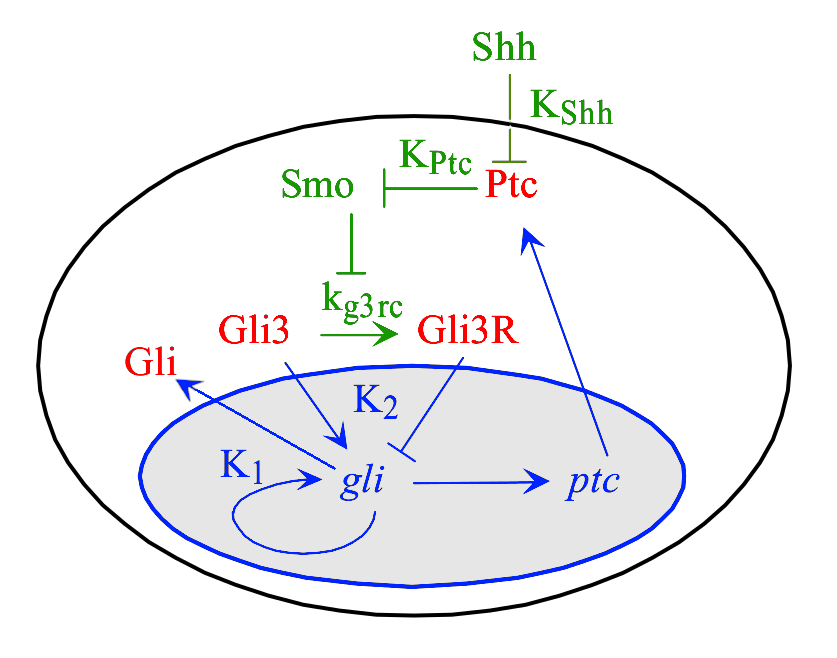
\includegraphics[width=0.85\linewidth]{signal_path_colors} 
	
	Variables del sistema en \textbf{\textcolor{red}{rojo}. }
	\begin{enumerate}
		\item \textbf{\textcolor{darkgreen}{Aparece Shh} \textcolor{darkgreen}{en el medio extracelular.}}
		\item \textbf{\textcolor{darkgreen}{Shh se une con la proteína } \textcolor{red}{Ptc.}}
		\item \textbf{\textcolor{darkgreen}{Al unirse con Shh se separa de Smo. }}
		\item \textbf{\textcolor{darkgreen}{Smo inhibe el paso de activador }\textcolor{red}{ Gli3} \textcolor{darkgreen}{a represor }\textcolor{red}{ Gli3R}.}
		\item \textbf{\textcolor{blue}{Al haber muchos activadores} \textcolor{red}{Gli3} \textcolor{blue}{se produce el comienzo de la expresión de \textit{gli} y \textit{ptc} (Aquí aplicamos el BEWARE).}}
		\item \textbf{\textcolor{blue}{La célula crea más } \textcolor{red}{Gli y Ptc}.}
		\item \textbf{\textcolor{darkgreen}{El nuevo } \textcolor{red}{Ptc} \textcolor{darkgreen}{ se une a Smo e inhibe el proceso.}}

	\end{enumerate}
\end{multicols} 
}

%%%%%%%%%%%%%%%%%%%%%%%%%%%%%%%%%%%%%%%%%%%%%%%%%%%%%%%%%%%%%%%%%%%%%%%%%%%%%%
\headerbox{Métodos}{name=metod,column=3,span=1}{
	%%%%%%%%%%%%%%%%%%%%%%%%%%%%%%%%%%%%%%%%%%%%%%%%%%%%%%%%%%%%%%%%%%%%%%%%%%%%%%
\begin{center}
	\centering \textbf{Modelado}\par
\end{center} 


Usamos la ley de acción de masas y el enfoque del modelo clásico para Gli3 Y Gli3R.
\\

Para Gli y Ptc, usamos la estrategia BEWARE, donde obtenemos la dinámica de Gli y Ptc según la expresión que tengamos de los genes que los codifican. 

Para ello se sigue el esquema:
\\

\centering
\includegraphics[height=0.3\textheight]{BEWARE}\\
		
		\textbf{Simulaciones (Código liberado)}
		\begin{itemize}
			\item AUTO07-P vía XppAut: Bifurcaciones
			\item SciPy (Python): Integración Numérica
		\end{itemize}

}
%%%%%%%%%%%%%%%%%%%%%%%%%%%%%%%%%%%%%%%%%%%%%%%%%%%%%%%%%%%%%%%%%%%%%%%%%%%%%%
\headerbox{Conclusiones}{name=concu,column=3,span=1, below = metod}{
	%%%%%%%%%%%%%%%%%%%%%%%%%%%%%%%%%%%%%%%%%%%%%%%%%%%%%%%%%%%%%%%%%%%%%%%%%%%%%%
\begin{itemize}
	\item Nuevas causas para la biestabilidad del modelo clásico.
	\item Nuevo modelo con un nuevo enfoque BEWARE más fiel a la realidad biológica.
	\item Ponemos en relevancia:
	\begin{itemize}
		\item La necesidad de seguir estudiando el modelo presentado
		\item La importancia de usar el nuevo enfoque BEWARE cuando modelamos procesos de regulación génica. 
	\end{itemize}

\end{itemize}
}

 %%%%%%%%%%%%%%%%%%%%%%%%%%%%%%%%%%%%%%%%%%%%%%%%%%%%%%%%%%%%%%%%%%%%%%%%%%%%%%
   \headerbox{Bibliografía}{name=references,column=0,span = 3, above=bottom}{
 %%%%%%%%%%%%%%%%%%%%%%%%%%%%%%%%%%%%%%%%%%%%%%%%%%%%%%%%%%%%%%%%%%%%%%%%%%%%%%
     \smaller
     \begin{multicols}{2}
     \bibliographystyle{apa}
\renewcommand{\section}[2]{\vskip 0.05em}
\begin{thebibliography}{1}\itemsep=-0.01em
	\setlength{\baselineskip}{0.4em}
	
	\bibitem{amberg07:nicp}
	Lai, K., Robertson, M. J., and Schaffer, D. V.
	\newblock The sonic hedgehog signaling system as a bistable genetic switch.
	\newblock In {\em Biophysical Journal}, 2004.
	\itemsep=-0.01em
	\setlength{\baselineskip}{0.4em}
	
	\bibitem{amberg07:nicp}
	M.~Cambon, O.~Sanchez.
	\newblock Analysis of biochemical mechanisms provoking differential spatial expression in Hh target genes.
	\newblock In {\em BioArxiv} 2017.
	
\end{thebibliography}
     \end{multicols}

   }

 %%%%%%%%%%%%%%%%%%%%%%%%%%%%%%%%%%%%%%%%%%%%%%%%%%%%%%%%%%%%%%%%%%%%%%%%%%%%%%


 %%%%%%%%%%%%%%%%%%%%%%%%%%%%%%%%%%%%%%%%%%%%%%%%%%%%%%%%%%%%%%%%%%%%%%%%%%%%%%



\end{poster}%
%
\end{document}
